% ------------------------------------------------------------------------
% file `main-bookexercise-8-exercise-body.tex'
%
%     exercise of type `bookexercise' with id `8'
%
% generated by the `exercise' environment of the
%   `xsim' package v0.21 (2022/02/12)
% from source `main' on 2026/10/30 on line 654
% ------------------------------------------------------------------------
1. 对于一个有$N$（$N>0$）个顶点的无向连通图，下列说法错误的是\underline{\hspace{1cm}}\\[0.5em]
A. 其最小生成树一定唯一\\
B. 其最小生成树可能不唯一\\
C. 其最小生成树一定有$N$个顶点\\
D. 其最小生成树一定有$N-1$条边\\

2. 下列说法正确的是\underline{\hspace{1cm}}\\[0.5em]
A. 对同一个图，Kruskal算法和Prim算法得到的最小生成树一定相同\\
B. 只要无向连通图中没有权值相同的边，其最小生成树一定唯一\\
C. 只要无向连通图中有权值相同的边，其最小生成树一定不唯一\\
D. 地球的体积比太阳大\\

3. 使用Kruskal算法求解下图的最小生成树，依次选取的边的顺序是什么？

\begin{center}
    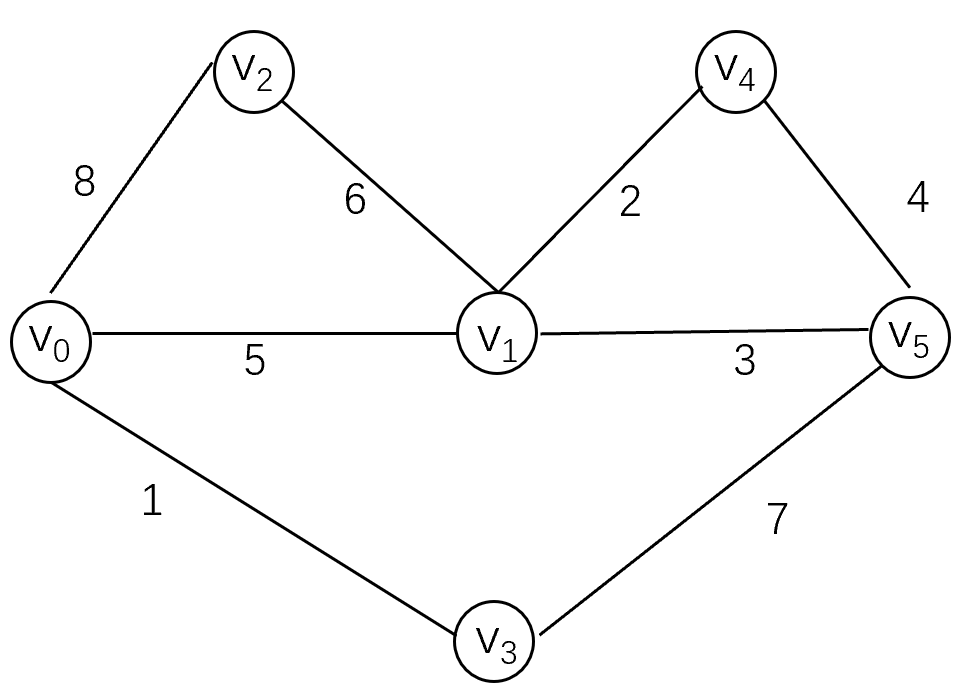
\includegraphics[width=0.39\textwidth]{assets/pics_and_ppts/ch5/习题13Kruskal选边顺序.png}
\end{center}

4. 下图是某个隐去了边权的无向连通图，现在用Kruskal算法求解其最小生成树，假设现在已经收入了(A, B)和(A, C)两条边，
则下一个收入的边绝不可能是\underline{\hspace{1cm}}\\[0.5em]
\begin{center}
    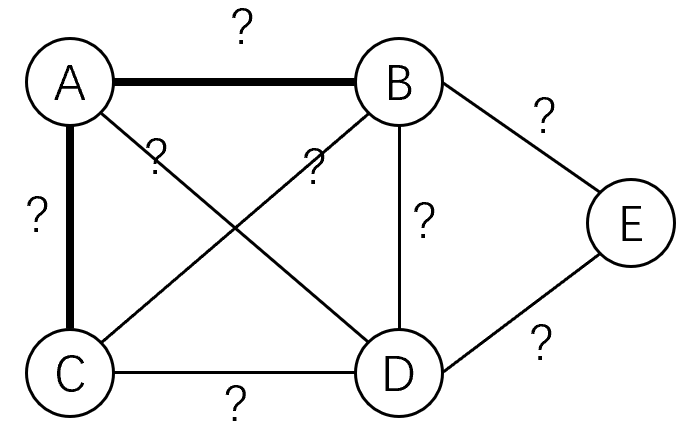
\includegraphics[width=0.33\textwidth]{assets/pics_and_ppts/ch5/习题14Kruskal不选已连通.png}
\end{center}

\begin{tabular}{llll}
    A. (B,C) & B. (B,D) & C. (C,D) & D. (D,E)
\end{tabular}

\vspace{\baselineskip}

5. （某年408真题）下列关于最小生成树的说法中，正确的是\underline{\hspace{1cm}}\\[0.5em]
\(\mathrm{I}\). 最小生成树的代价唯一\\
\(\mathrm{II}\). 所有权值最小的边一定会出现在所有的最小生成树中\\
\(\mathrm{III}\). 使用Prim算法从不同顶点开始得到的最小生成树一定相同\\
\(\mathrm{IV}\). 使用Prim算法和Kruskal算法得到的最小生成树总不相同\\

\noindent A. 仅\(\mathrm{I}\) \;\;\; B. 仅\(\mathrm{II}\) \;\;\; C. 仅\(\mathrm{I}\)、\(\mathrm{III}\) \;\;\; D. 仅\(\mathrm{II}\)、\(\mathrm{IV}\)

\vspace{\baselineskip}

6. （某年408真题）求下面带权图的最小生成树时，可能是Kruskal算法第2次选中但一定不是Prim算法（从d开始）第2次选中的边的是\underline{\hspace{1cm}}\\[0.5em]

\begin{center}
    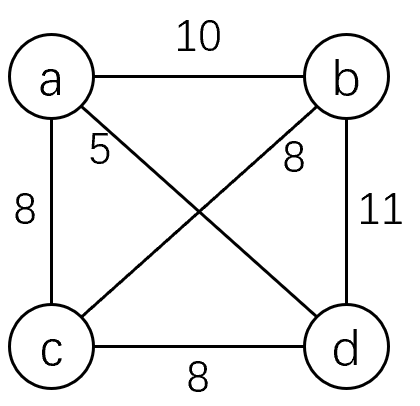
\includegraphics[width=0.20\textwidth]{assets/pics_and_ppts/ch5/习题16，15408Prim与Kruskal第二次选边.png}
\end{center}

\begin{tabular}{llll}
    A. (a, c) & B. (a, d) & C. (b, c) & D. (c, d)
\end{tabular}

\vspace{\baselineskip}

7. 对下图所示的有向无环图进行拓扑排序，不可能得到的拓扑序列是\underline{\hspace{1cm}}\\

\begin{center}
    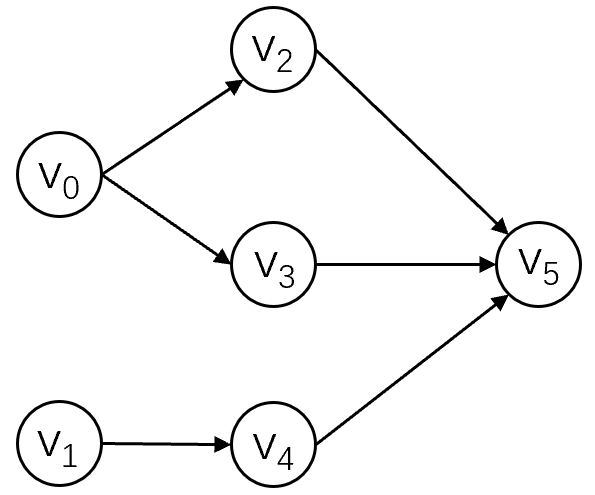
\includegraphics[width=0.25\textwidth]{assets/pics_and_ppts/ch5/习题16，拓扑排序可能的序列.png}
\end{center}

\begin{tabular}{ll}
    A. $v_0, v_1, v_2, v_3, v_4, v_5$ & B. $v_1, v_0, v_4, v_3, v_2, v_5$ \\
    C. $v_0, v_1, v_4, v_3, v_2, v_5$ & D. $v_1, v_0, v_5, v_4, v_3, v_2$
\end{tabular}

\vspace{\baselineskip}

8. （某年408真题）对下图所示的有向无环图进行拓扑排序，可能得到\underline{\hspace{1cm}}个不同的拓扑序列\\

\begin{center}
    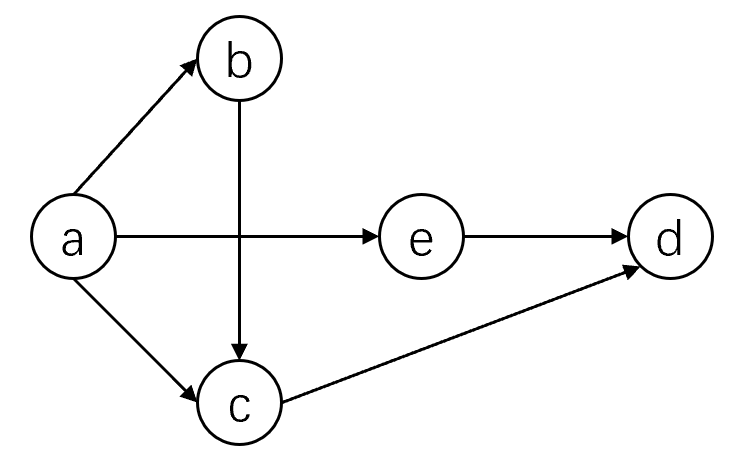
\includegraphics[width=0.35\textwidth]{assets/pics_and_ppts/ch5/习题17，21408拓扑排序可能的序列数量.png}
\end{center}

\begin{tabular}{llll}
    A. 1 & B. 2 & C. 3 & D. 4
\end{tabular}

\vspace{\baselineskip}

9. 对于有向图无环图$G$的一个拓扑序列，若顶点$v_1$在顶点$v_3$之前，请判断下列命题的正确性。\\[0.5em]
A. 一定存在有向边：$(v_1, v_3)$\\
B. 可能存在有向边：$(v_3, v_1)$\\
C. 一定存在一条从$v_1$到$v_3$的路径\\
D. 可能存在一条从$v_3$到$v_1$的路径\\
E. 可能存在一条从$v_1$到$v_3$的路径\\

10. 对于下图所示的AOE网，其关键路径长度的是\underline{\hspace{1cm}}\\[0.5em]
\begin{center}
    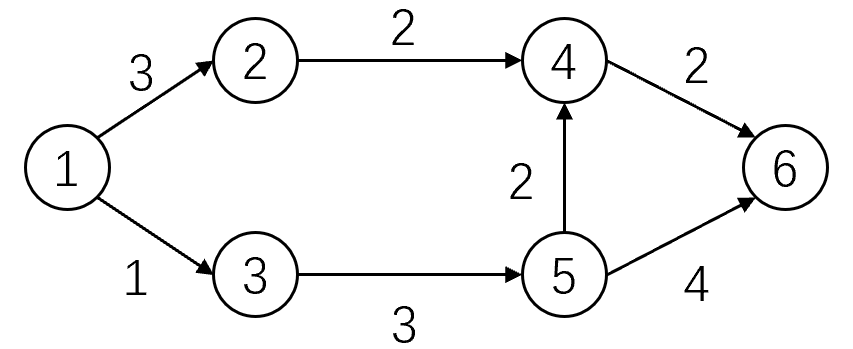
\includegraphics[width=0.40\textwidth]{assets/pics_and_ppts/ch5/习题19关键路径长度练习.png}
\end{center}
\begin{tabular}{llll}
    A. 6 & B. 7 & C. 8 & D. 9
\end{tabular}

\vspace{\baselineskip}

11. （某年408真题）若使用AOE网估算工程进度，下列叙述中正确的是\underline{\hspace{1cm}}\\[0.5em]
A. 关键路径是从源点到汇点边数最多的一条路径\\
B. 关键路径是从源点到汇点路径长度最长的一条路径\\
C. 增加任意一个关键活动的时间不会延长工程的工期\\
D. 缩短任意一个关键活动的时间将会缩短工程的工期\\


12. （某年408真题）下列AOE网表示一项包含8个活动的工程。则同时加快\underline{\hspace{1cm}}中的两个活动就可以缩短工程工期\\[0.5em]

\begin{center}
    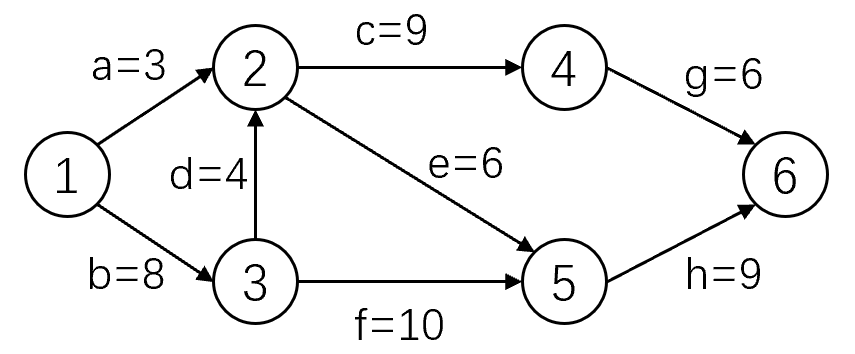
\includegraphics[width=0.36\textwidth]{assets/pics_and_ppts/ch5/习题20，13408同时加快活动缩短工期.png}
\end{center}

\begin{tabular}{llll}
    A. c和e & B. d和c & C. f和d & D. f和h
\end{tabular}

\vspace{\baselineskip}

13. 经历了一场战争后，王国的一些道路遭到了严重破坏。国王决定重建城市之间的道路，使得所有城市重新连通。
王国共有 N 座城市，编号为 0 到 N-1。工程师经过地质考察，给出了 M 条可以修建的道路，每条道路连接两座不同的城市，并给出了修建这条道路所需的费用。
此外，部分城市之间已经存在完好的旧道路。这些旧道路可以直接使用，不需要重新修建。

给出所有尚存的旧道路（保证不存在环）和可以修建的道路，请你帮助国王计算：在保证任意两座城市之间都能够互相到达的前提下，至少还需要花费多少费用？
如果无论如何都无法使所有城市连通，则返回 -1。

\begin{cppcode}
    struct Road {
        int u, v;   // 道路连通的两个城市编号
    };
    struct NewRoad {
        int u, v;   // 修建该道路后，将连通的两个城市的编号
        int weight; // 修建该道路需要的花费
    };
    int minimumCost(
        int N,
        vector<Road>& existing_roads,
        vector<NewRoad> new_roads
    ) {

    }
\end{cppcode}

\vspace{\baselineskip}

14.
王国的重建工程被划分为 N 项任务，编号为 0 到 N-1。
然而，部分任务之间存在先后依赖关系。例如，必须先完成地基施工，才能开始墙体建设；必须先完成墙体建设，才能安装城堡屋顶。
工程师整理出了 M 条任务依赖关系。每条依赖关系由两个整数 u 和 v 表示，意味着任务 u 必须在任务 v 之前完成。
请你帮助国王安排这 N 项任务的执行顺序，使得所有任务都能按照依赖关系完成，返回代表任务执行顺序的数组。
如果存在任务依赖关系上的矛盾，导致所有任务无法安排出一个合法的执行顺序，则返回一个空数组。
如果存在多种合法的执行顺序，返回其中任意一种即可。

\begin{cppcode}
    // v1、v2的长度均为M，用于表示任务的依赖关系：对于 0 <= i < M, 任务 v1[i] 必须在 v2[i]之前完成。
    vector<int> TopologicalSort(int N, int M, vector<int>& v1, vector<int>& v2) {

    }
\end{cppcode}

\vspace{\baselineskip}

*15. 王国的重建工程有 N 项任务，编号为 $1,2,\ldots,N$。为了尽快完成不同任务，各方工作人员可以同时进行多项互不冲突的任务。
对于第 $i$ 项任务：\\
- 完成它需要花费 $T_i$ 个时间单位。\\
- 在开始第 $i$ 项任务之前，必须先完成若干项指定的任务。\\
- 如果某项任务没有前置依赖，那么它可以立即开始。

给出$T[]$以及每项任务的直接前置依赖Pre[]，请你计算：完成全部 $N$ 项任务，最少需要多少时间（保证依赖关系不存在矛盾）？


\begin{cppcode}
    // T[]与Pre[]长度均为N，T[i]表示任务 i 的花费时间；Pre[i] 表示任务 i 的所有直接前置依赖
    int MinTime(int N, int T[], vector<int> Pre[]) {

    }
\end{cppcode}


